\chapter{Results}
\label{chap:Results}

\section{Performance Across Annotation Budgets}
We compare seven uncertainty-based strategies with random sampling using five seeds and ten annotation budgets, from approximately 10\% to 100\%. Each round trains F$^3$ED from scratch and selects the checkpoint with the highest validation edit score. All results below use the held-out test set. Within each seed, strategies share the same initial labeled pool and identical initial and full-budget scores.

The figures show means and one sample standard deviation across seeds. Their vertical axes are cropped to reveal differences; within each metric, panel heights preserve the same score units per vertical distance. The tables report AULC on a 0--100 scale, with relative changes from random sampling in parentheses. Rankings describe these five runs and do not establish statistical significance.

\subsection{Mean F1 Event}

All seven strategies improve event-F1 AULC over random sampling at $G_{\mathrm{high}}$ and $G_{\mathrm{mid}}$ (Table~\ref{tab:aulc_f1_event}). Each improvement is positive in all five paired seeds. Weighted EM achieves the largest mean gains: 2.27 and 2.86 AULC points, or 6.10\% and 6.29\%, respectively. At $G_{\mathrm{low}}$, gains are smaller, and both ungrouped fine strategies fall below the baseline on average.

The budget crossings illustrate the practical difference. Weighted EM first reaches 95\% of the full-budget mean event F1 at approximately 30\% annotation for both high and medium granularity. Random sampling first reaches these targets at approximately 50\% and 60\%, respectively. These are observed crossings of the mean curves, not estimates of the minimum budget required in every run.

Several strategies also exceed the full-budget event F1 at intermediate budgets. For example, Weighted EM reaches 0.427 at approximately 80\% annotation at $G_{\mathrm{high}}$, compared with 0.407 at full budget. Changing sample composition under a fixed training schedule could contribute to this behavior. The results alone do not show that the remaining samples are harmful or that more data generally reduces performance.

\begin{figure}[htbp]
    \centering
    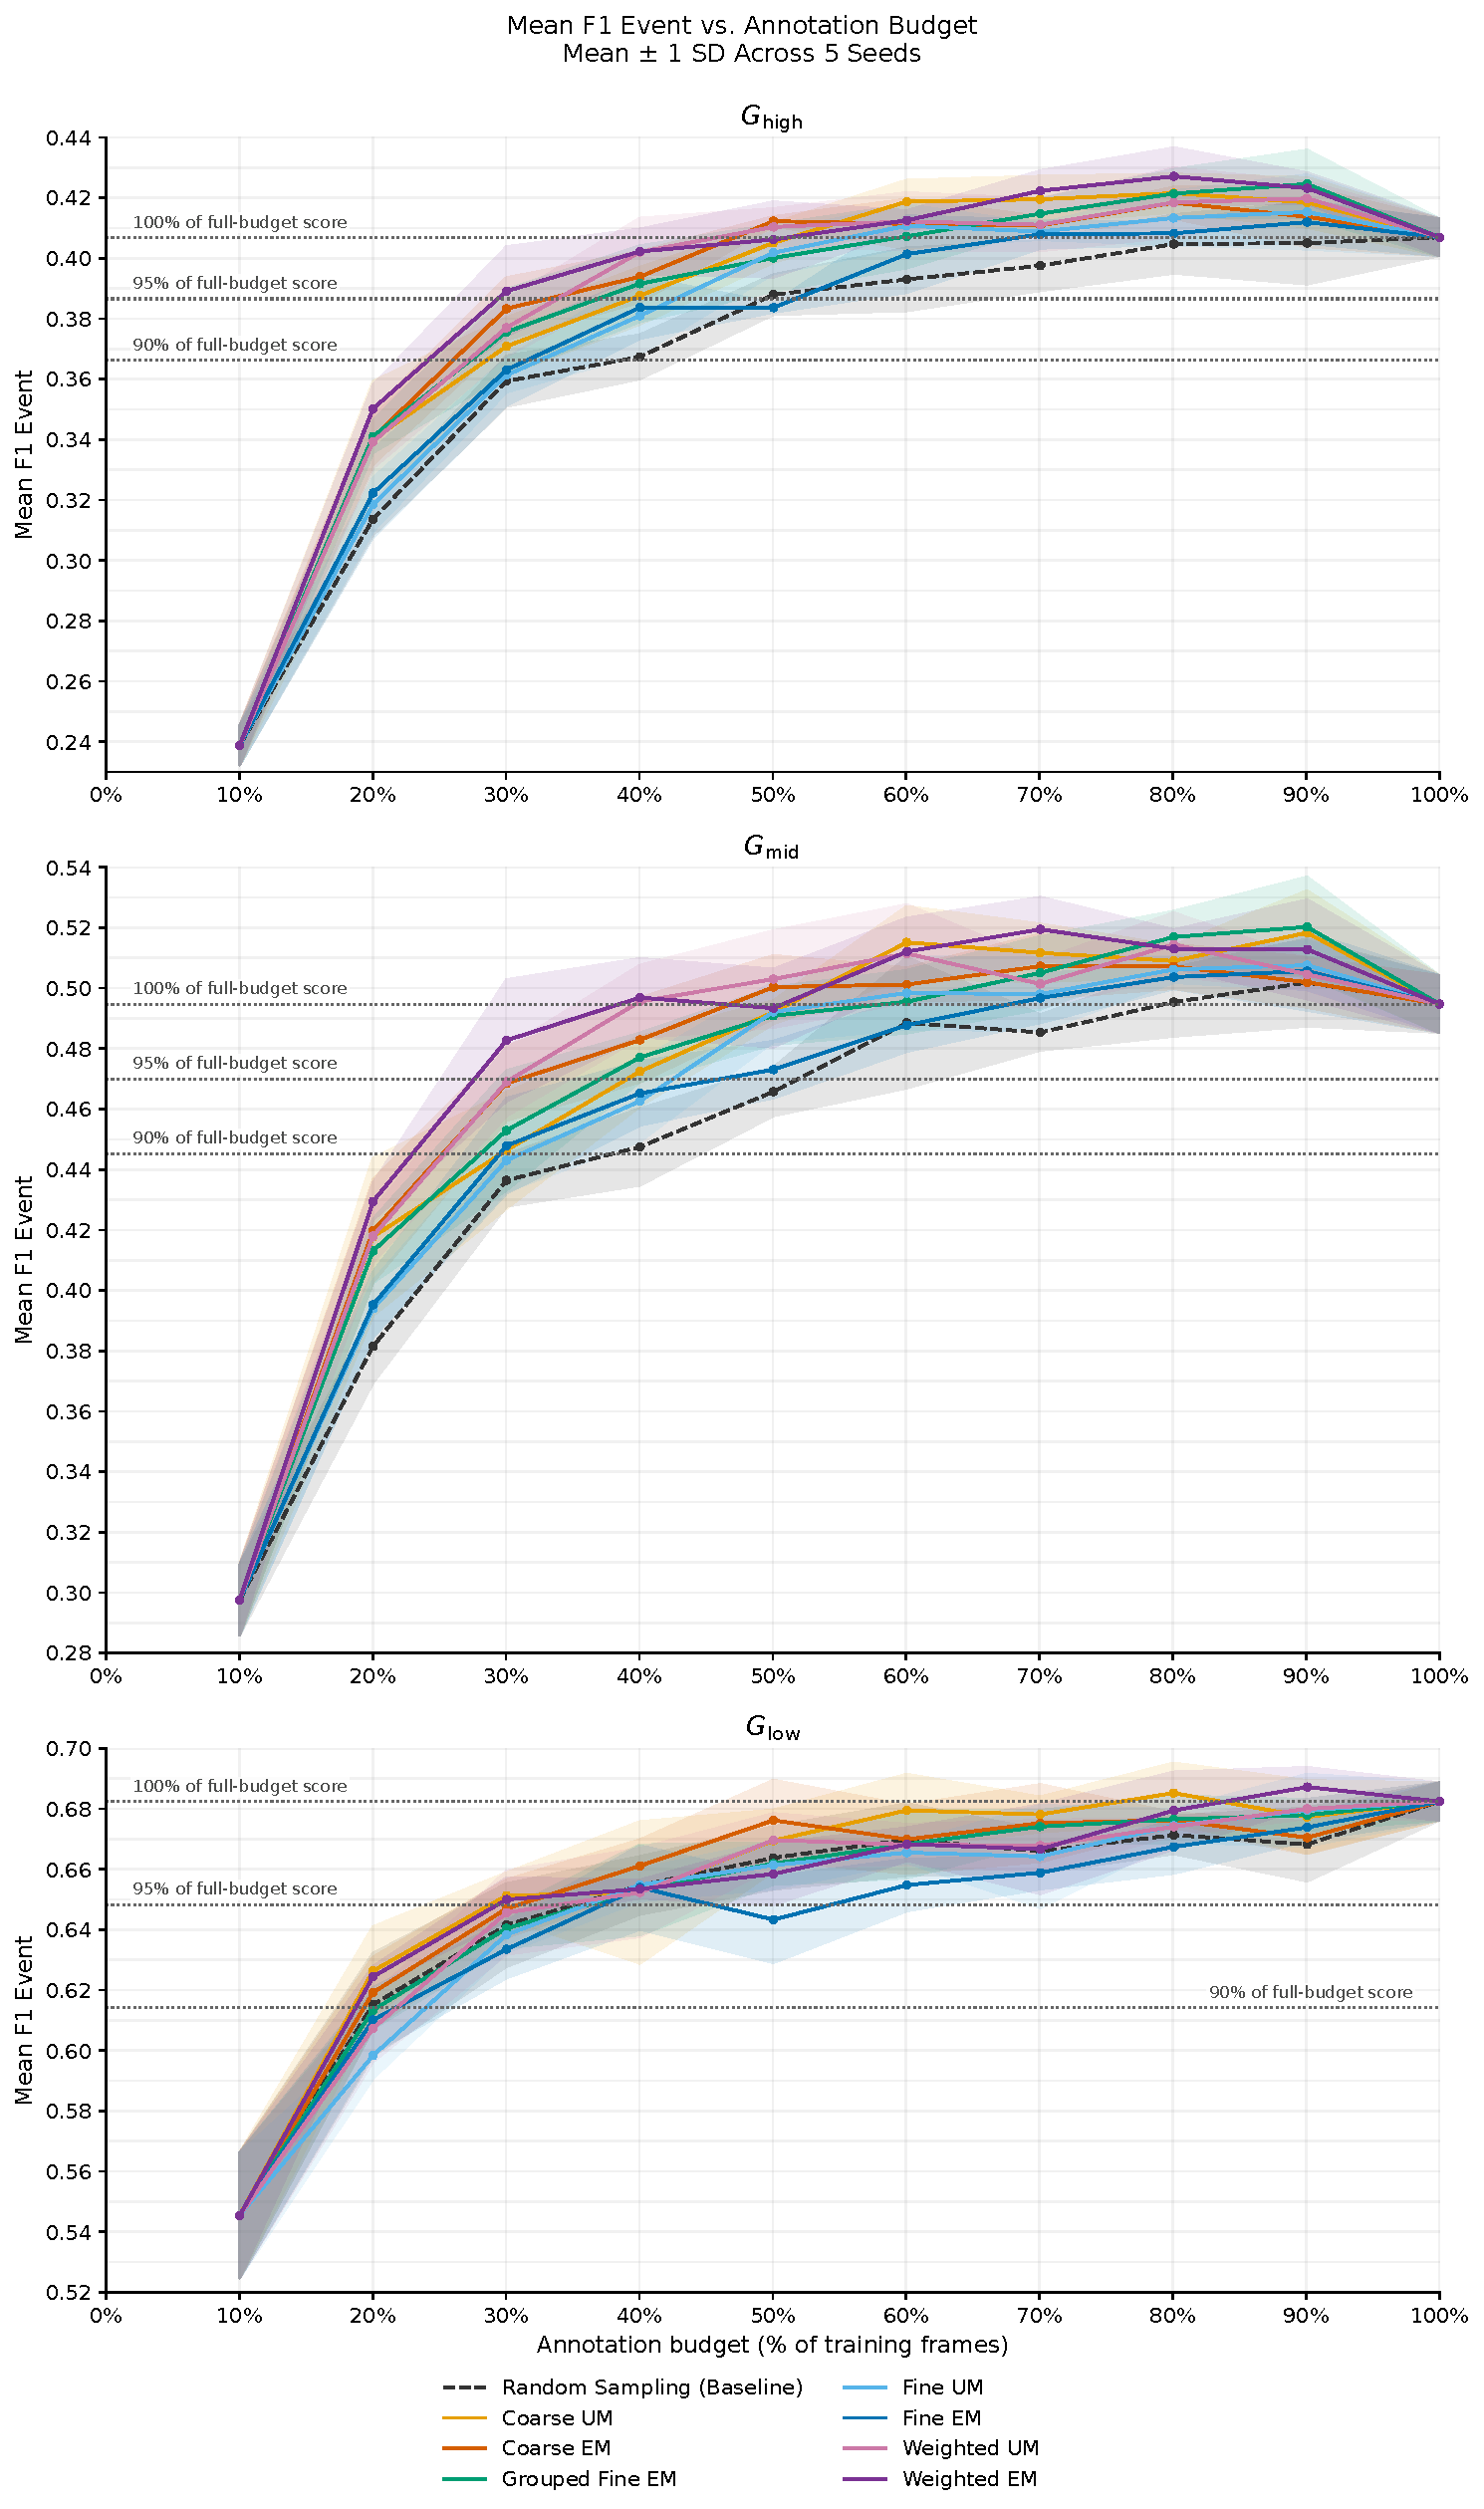
\includegraphics[width=0.85\textwidth,height=0.78\textheight,keepaspectratio]{figures/learning_curves_test_f1_event.pdf}
    \caption{Event F1 across annotation budgets. Lines show means and bands show one sample standard deviation across five seeds. Dotted lines mark fractions of the full-budget mean. Vertical axes are cropped.}
    \label{fig:Learning Curves (Mean F1 Event)}
\end{figure}


\begin{table}[htbp]
    \centering
    \caption{AULC across query strategies and label granularities. Values are mean $\pm$ sample standard deviation across five seeds, with relative changes from random sampling in parentheses. The largest mean gain per column is bolded.}
    \label{tab:aulc_f1_event}
    \small
    \begin{adjustbox}{max width=\textwidth}
        \begin{tabular}{lccc}
            \toprule
            \multicolumn{4}{c}{\textbf{AULC (Mean F1 Event)}} \\
            \cmidrule(lr){1-4}
            \textbf{Query Strategy} & $\boldsymbol{G_{\mathrm{high}}}$ & $\boldsymbol{G_{\mathrm{mid}}}$ & $\boldsymbol{G_{\mathrm{low}}}$ \\
            \midrule
            R. Sampling (Baseline) & 37.23 $\pm$ 0.25 (+0.00\%) & 45.53 $\pm$ 0.32 (+0.00\%) & 65.16 $\pm$ 0.50 (+0.00\%) \\
            Coarse UM               & 38.94 $\pm$ 0.43 (+4.58\%) & 47.54 $\pm$ 0.70 (+4.41\%) & 65.93 $\pm$ 0.41 (\textbf{+1.18\%}) \\
            Coarse EM               & 38.96 $\pm$ 0.43 (+4.65\%) & 47.61 $\pm$ 0.53 (+4.56\%) & 65.66 $\pm$ 0.14 (+0.77\%) \\
            Fine UM                 & 38.15 $\pm$ 0.30 (+2.45\%) & 46.64 $\pm$ 0.45 (+2.44\%) & 65.00 $\pm$ 0.32 (-0.24\%) \\
            Fine EM                 & 37.83 $\pm$ 0.19 (+1.60\%) & 46.34 $\pm$ 0.35 (+1.78\%) & 64.55 $\pm$ 0.33 (-0.93\%) \\
            Grouped Fine EM         & 38.87 $\pm$ 0.28 (+4.41\%) & 47.42 $\pm$ 0.50 (+4.14\%) & 65.33 $\pm$ 0.46 (+0.26\%) \\
            Weighted UM             & 39.03 $\pm$ 0.28 (+4.83\%) & 47.93 $\pm$ 0.17 (+5.26\%) & 65.32 $\pm$ 0.59 (+0.25\%) \\
            Weighted EM             & 39.50 $\pm$ 0.33 (\textbf{+6.10\%}) & 48.40 $\pm$ 0.57 (\textbf{+6.29\%}) & 65.57 $\pm$ 0.28 (+0.64\%) \\
            \bottomrule
        \end{tabular}
    \end{adjustbox}
\end{table}

\subsection{Mean F1 Element}

Element-F1 results broadly follow event F1, with Weighted EM leading at high and medium granularity (Table~\ref{tab:aulc_f1_element}). However, its gains are smaller: 1.07 and 1.18 AULC points. Element F1 credits individual correct attributes, while event F1 requires the complete combination to be correct. Improvements in attribute predictions may therefore have a larger effect on complete-event recognition. The different averaging units also prevent a direct comparison of the two metrics' absolute scores.

At low granularity, the best improvement is only 0.35 AULC points, from Coarse UM. As with event F1, Fine UM and Fine EM score below random sampling. Thus, using more detailed attribute uncertainty does not necessarily improve the coarser evaluation target.


\begin{figure}[htbp]
    \centering
    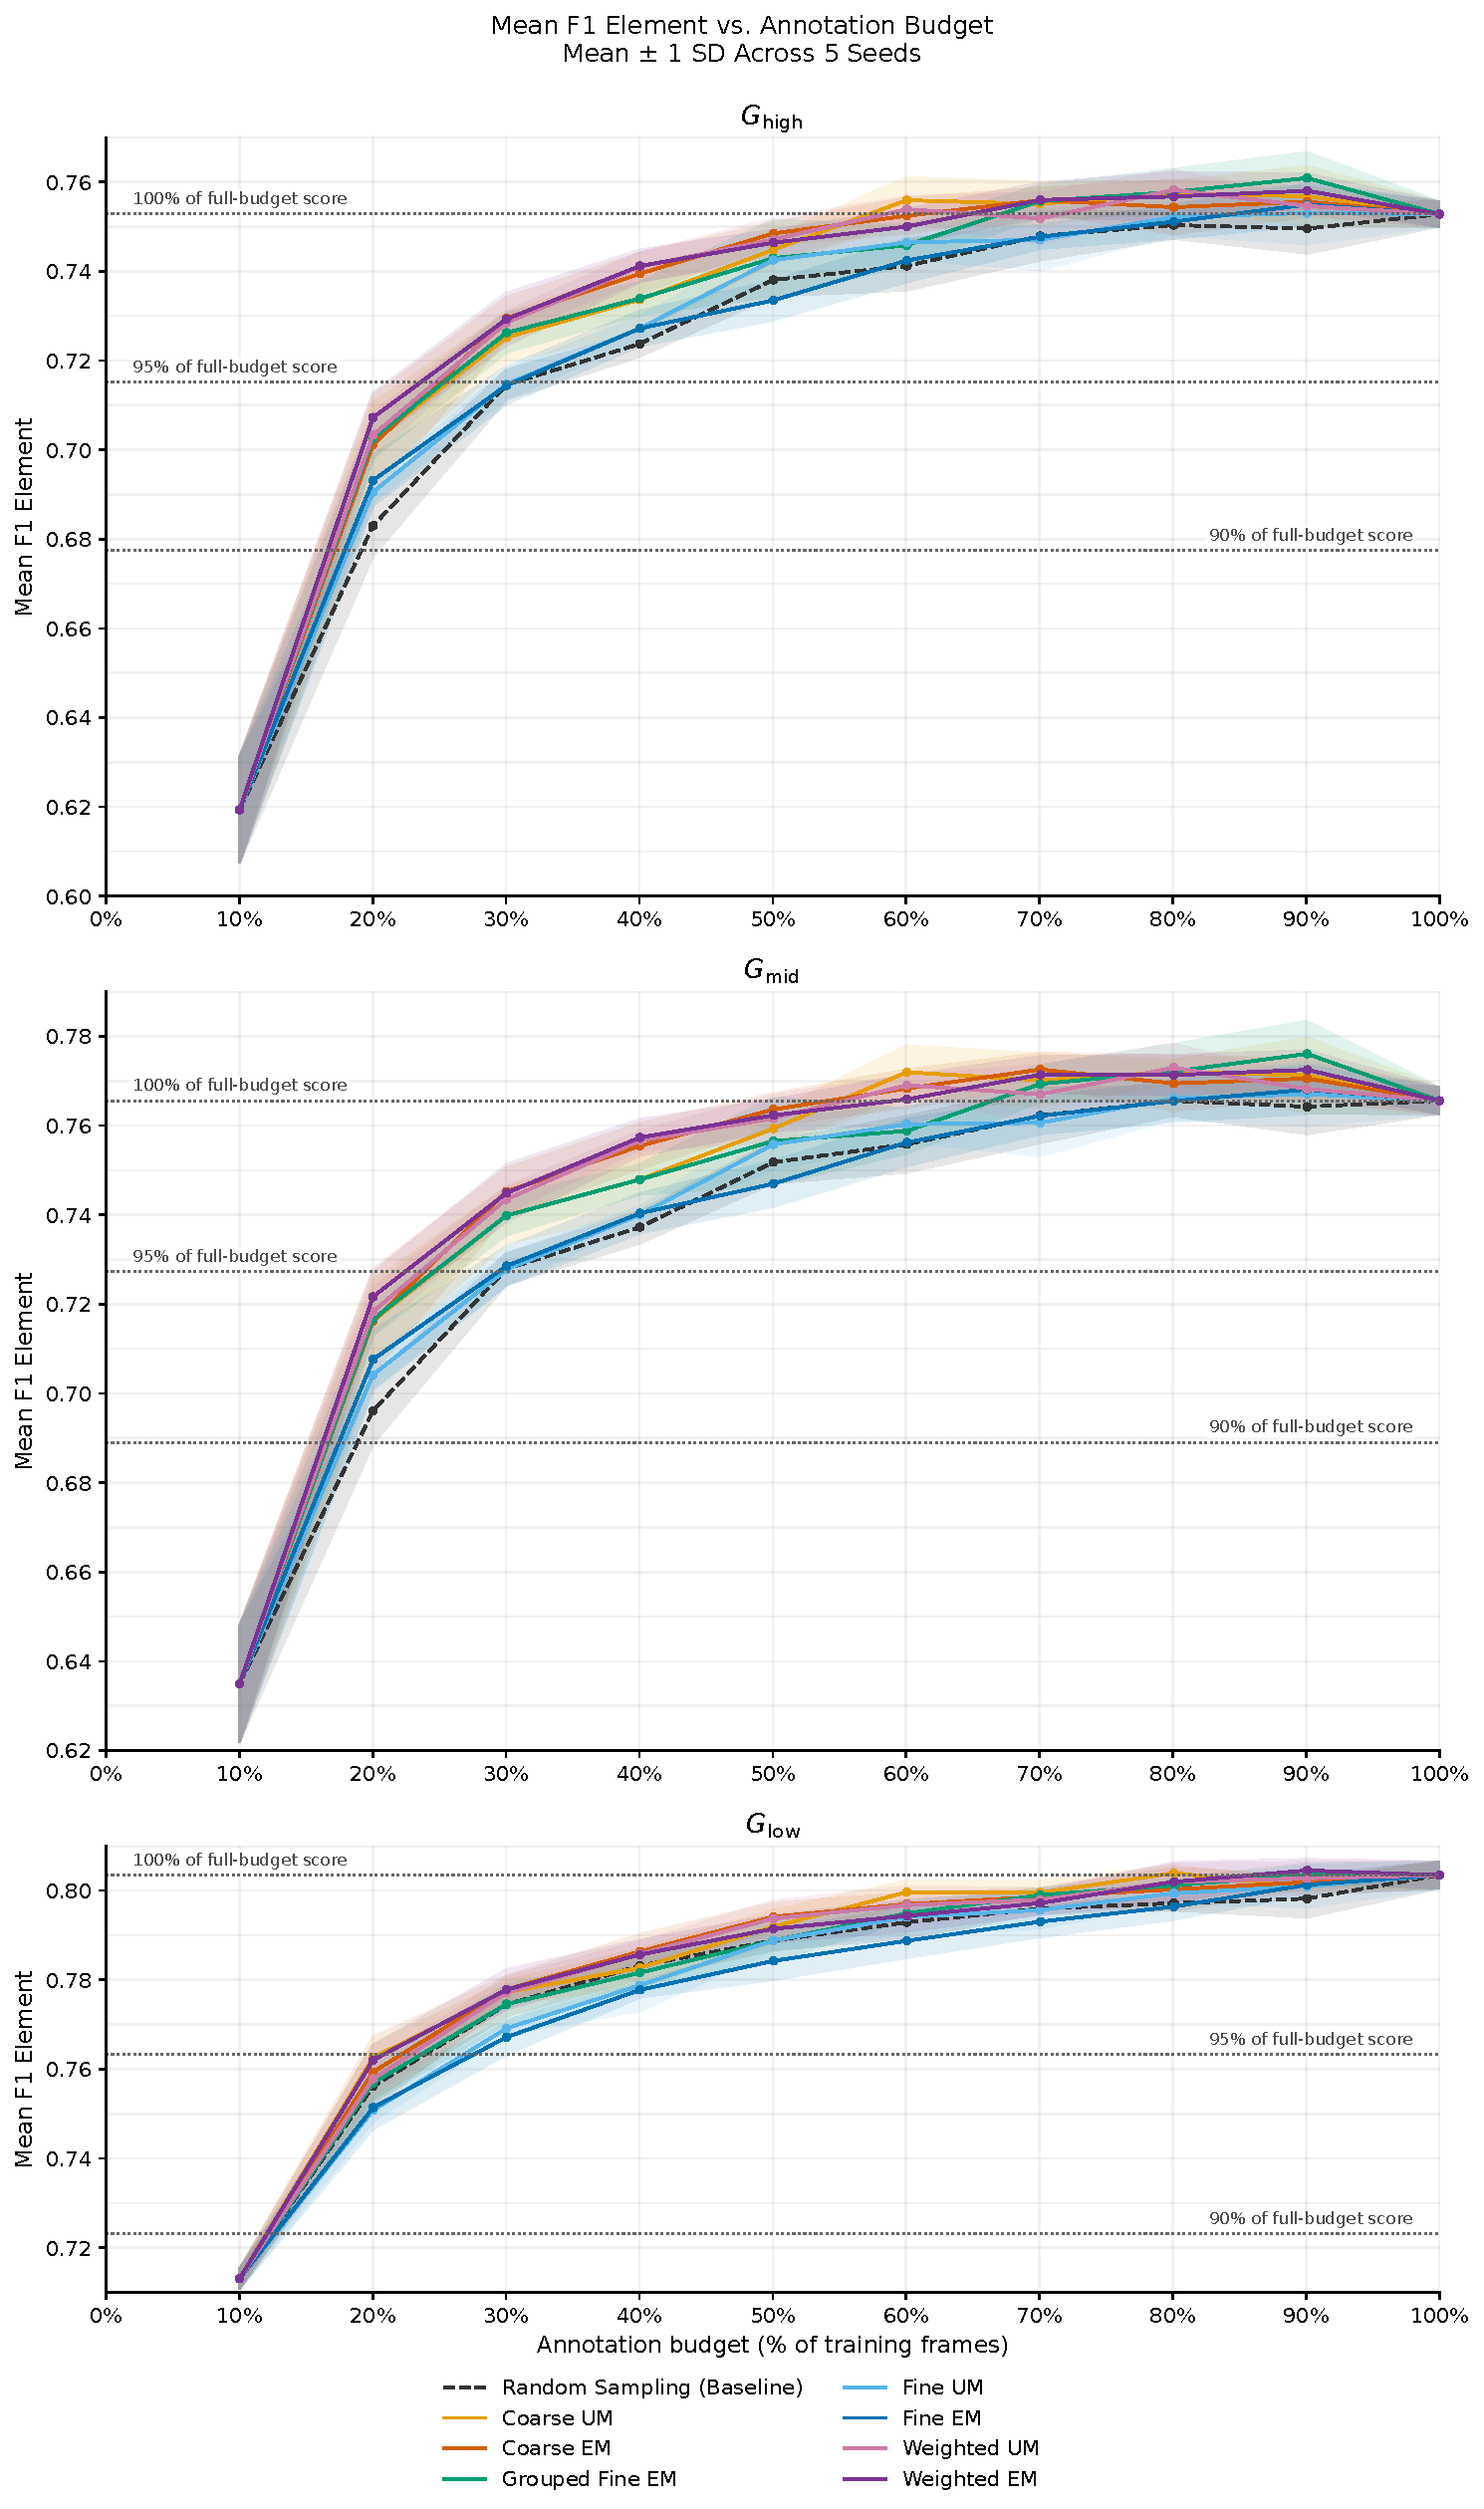
\includegraphics[width=0.85\textwidth,height=0.78\textheight,keepaspectratio]{figures/learning_curves_test_f1_element.pdf}
    \caption{Element F1 across annotation budgets. Lines show means and bands show one sample standard deviation across five seeds. Dotted lines mark fractions of the full-budget mean. Vertical axes are cropped.}
    \label{fig:Learning Curves (Mean F1 Element)}
\end{figure}

\begin{table}[htbp]
    \centering
    \caption{AULC across query strategies and label granularities. Values are mean $\pm$ sample standard deviation across five seeds, with relative changes from random sampling in parentheses. The largest mean gain per column is bolded.}
    \label{tab:aulc_f1_element}
    \small
    \begin{adjustbox}{max width=\textwidth}
        \begin{tabular}{lccc}
            \toprule
            \multicolumn{4}{c}{\textbf{AULC (Mean F1 Element)}} \\
            \cmidrule(lr){1-4}
            \textbf{Query Strategy} & $\boldsymbol{G_{\mathrm{high}}}$ & $\boldsymbol{G_{\mathrm{mid}}}$ & $\boldsymbol{G_{\mathrm{low}}}$ \\
            \midrule
            R. Sampling (Baseline) & 72.60 $\pm$ 0.13 (+0.00\%) & 74.01 $\pm$ 0.15 (+0.00\%) & 78.28 $\pm$ 0.09 (+0.00\%) \\
            Coarse UM               & 73.52 $\pm$ 0.33 (+1.26\%) & 74.99 $\pm$ 0.37 (+1.32\%) & 78.63 $\pm$ 0.14 (\textbf{+0.45\%}) \\
            Coarse EM               & 73.59 $\pm$ 0.33 (+1.36\%) & 75.13 $\pm$ 0.34 (+1.51\%) & 78.60 $\pm$ 0.17 (+0.41\%) \\
            Fine UM                 & 72.88 $\pm$ 0.16 (+0.39\%) & 74.24 $\pm$ 0.20 (+0.31\%) & 78.17 $\pm$ 0.05 (-0.13\%) \\
            Fine EM                 & 72.78 $\pm$ 0.09 (+0.25\%) & 74.17 $\pm$ 0.13 (+0.22\%) & 77.98 $\pm$ 0.05 (-0.38\%) \\
            Grouped Fine EM         & 73.46 $\pm$ 0.10 (+1.19\%) & 74.86 $\pm$ 0.12 (+1.15\%) & 78.43 $\pm$ 0.15 (+0.19\%) \\
            Weighted UM             & 73.60 $\pm$ 0.05 (+1.38\%) & 75.08 $\pm$ 0.09 (+1.45\%) & 78.58 $\pm$ 0.08 (+0.38\%) \\
            Weighted EM             & 73.67 $\pm$ 0.22 (\textbf{+1.48\%}) & 75.19 $\pm$ 0.25 (\textbf{+1.60\%}) & 78.59 $\pm$ 0.18 (+0.40\%) \\
            \bottomrule
        \end{tabular}
    \end{adjustbox}
\end{table}

\subsection{Edit Score}

Higher event F1 does not consistently translate into higher edit score (Table~\ref{tab:aulc_edit}). Coarse and weighted strategies lose edit-score AULC at high and low granularity in all five paired seeds. At medium granularity, their mean gains are small. Fine UM has the highest mean edit-score AULC at high and low granularity, while Grouped Fine EM leads at medium granularity.

These metrics reward different aspects of a prediction. A more accurately timed event can improve exact-frame F1 without changing its position in the event sequence. Event F1 also averages over classes, whereas edit score averages over clips. Improvements can therefore be distributed differently across the two metrics.

The granularity pattern is also relevant: $G_{\mathrm{low}}$ includes shot outcome, which $G_{\mathrm{mid}}$ excludes; it is not a subset of $G_{\mathrm{mid}}$ \autocite{liu_f3set_2025}. Differences in the acquired outcome labels offer one possible explanation for the edit-score losses, examined in Section~\ref{sec:Comparison Between Query Strategies}. We cannot attribute them to outcome prediction errors without an error breakdown.

\begin{figure}[htbp]
    \centering
    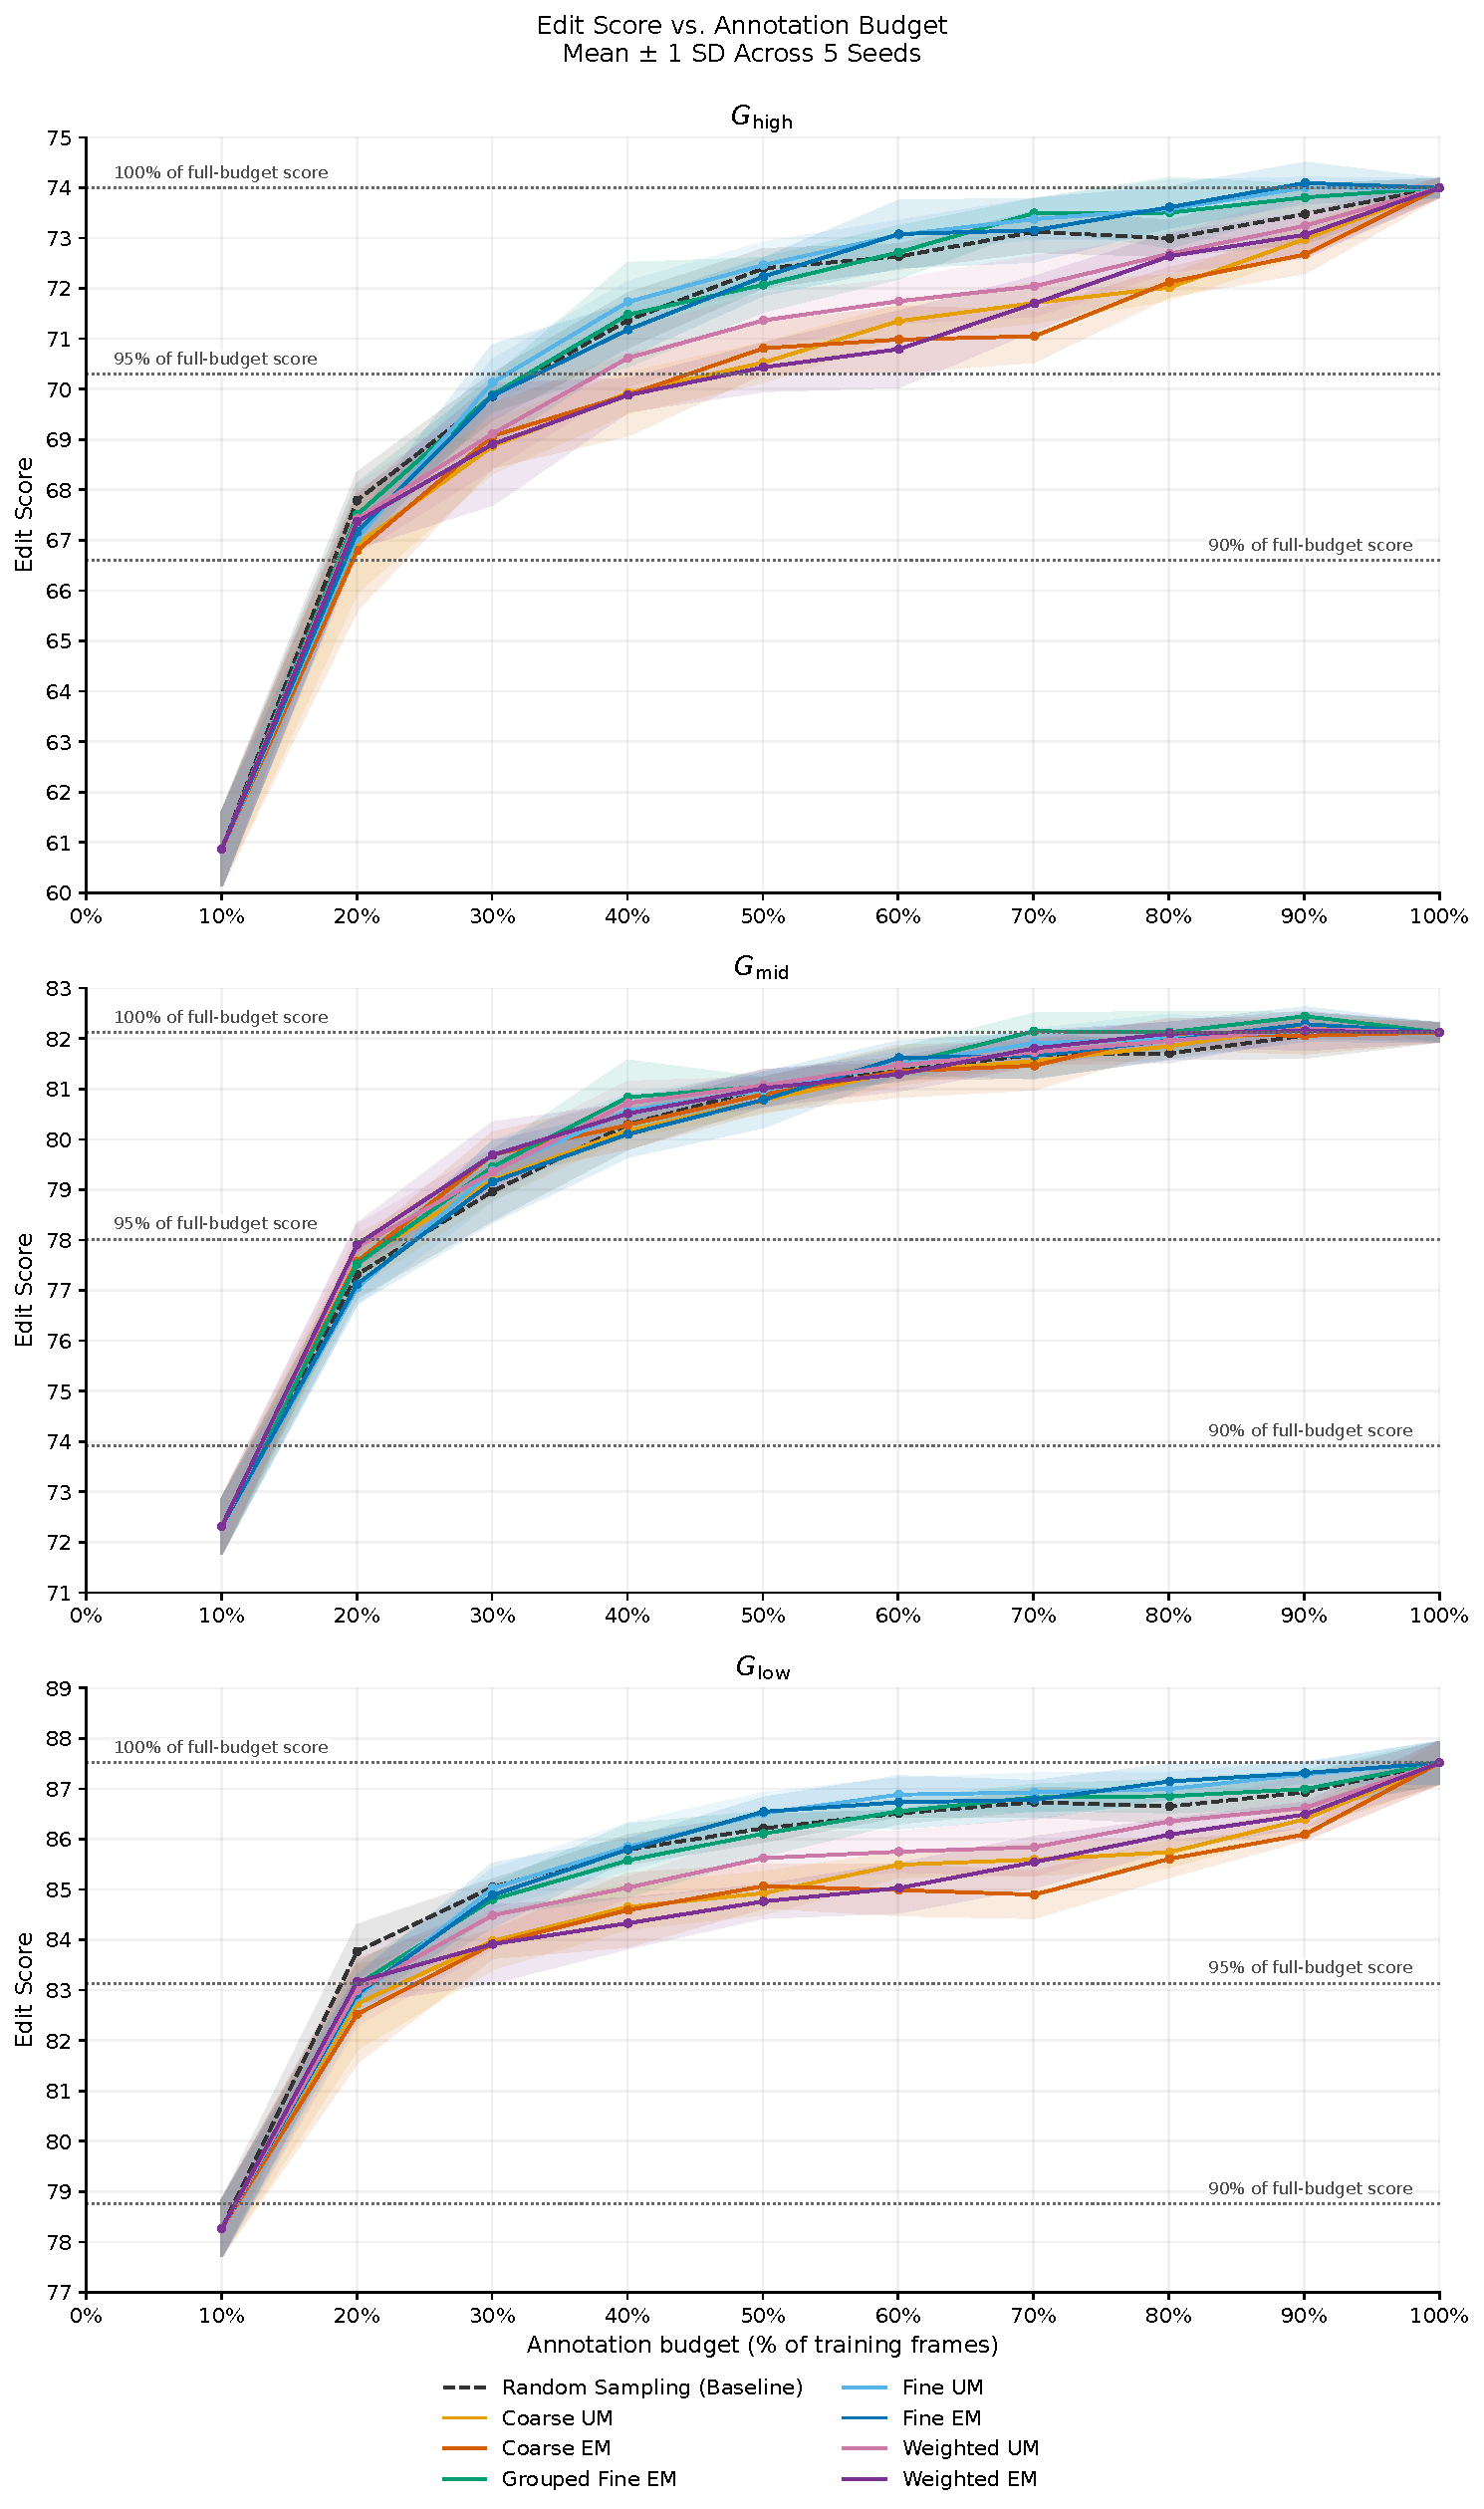
\includegraphics[width=0.85\textwidth,height=0.78\textheight,keepaspectratio]{figures/learning_curves_test_edit.pdf}
    \caption{Edit score across annotation budgets. Lines show means and bands show one sample standard deviation across five seeds. Dotted lines mark fractions of the full-budget mean. Vertical axes are cropped.}
    \label{fig:Learning Curves (Edit Score)}
\end{figure}

\begin{table}[htbp]
    \centering
    \caption{Edit-score AULC across query strategies and label granularities. Values are mean $\pm$ sample standard deviation across five seeds, with relative changes from random sampling in parentheses. The largest mean gain per column is bolded.}
    \label{tab:aulc_edit}
    \small
    \begin{adjustbox}{max width=\textwidth}
        \begin{tabular}{lccc}
            \toprule
            \multicolumn{4}{c}{\textbf{AULC (Edit Score)}} \\
            \cmidrule(lr){1-4}
            \textbf{Query Strategy} & $\boldsymbol{G_{\mathrm{high}}}$ & $\boldsymbol{G_{\mathrm{mid}}}$ & $\boldsymbol{G_{\mathrm{low}}}$ \\
            \midrule
            R. Sampling (Baseline) & 71.23 $\pm$ 0.07 (+0.00\%) & 80.18 $\pm$ 0.09 (+0.00\%) & 85.61 $\pm$ 0.08 (+0.00\%) \\
            Coarse UM               & 70.19 $\pm$ 0.21 (-1.46\%) & 80.21 $\pm$ 0.13 (+0.04\%) & 84.71 $\pm$ 0.17 (-1.06\%) \\
            Coarse EM               & 70.09 $\pm$ 0.42 (-1.60\%) & 80.29 $\pm$ 0.22 (+0.14\%) & 84.51 $\pm$ 0.30 (-1.29\%) \\
            Fine UM                 & 71.42 $\pm$ 0.14 (\textbf{+0.27\%}) & 80.30 $\pm$ 0.13 (+0.16\%) & 85.69 $\pm$ 0.14 (\textbf{+0.09\%}) \\
            Fine EM                 & 71.31 $\pm$ 0.31 (+0.12\%) & 80.21 $\pm$ 0.24 (+0.04\%) & 85.67 $\pm$ 0.14 (+0.06\%) \\
            Grouped Fine EM         & 71.32 $\pm$ 0.24 (+0.13\%) & 80.47 $\pm$ 0.20 (\textbf{+0.37\%}) & 85.52 $\pm$ 0.14 (-0.11\%) \\
            Weighted UM             & 70.63 $\pm$ 0.28 (-0.84\%) & 80.40 $\pm$ 0.23 (+0.27\%) & 85.06 $\pm$ 0.16 (-0.64\%) \\
            Weighted EM             & 70.24 $\pm$ 0.27 (-1.38\%) & 80.41 $\pm$ 0.14 (+0.29\%) & 84.69 $\pm$ 0.19 (-1.08\%) \\
            \bottomrule
        \end{tabular}
    \end{adjustbox}
\end{table}

\subsection{Mean F1 Class-Agnostic}

Coarse EM achieves the highest class-agnostic AULC, improving on random sampling by 0.57 points (Table~\ref{tab:aulc_class_agnostic}). Coarse UM and both weighted strategies also improve localization in all five paired seeds. In contrast, Fine UM and Fine EM fall below random sampling in every seed. Grouped Fine EM remains close to the baseline.

There is only one class-agnostic curve per strategy because event locations are shared across granularities. These results suggest that explicitly using event presence helps localization. The gains are modest relative to the already high baseline, but this does not establish that active learning is generally ineffective for simpler tasks.


\begin{figure}[htbp]
    \centering
    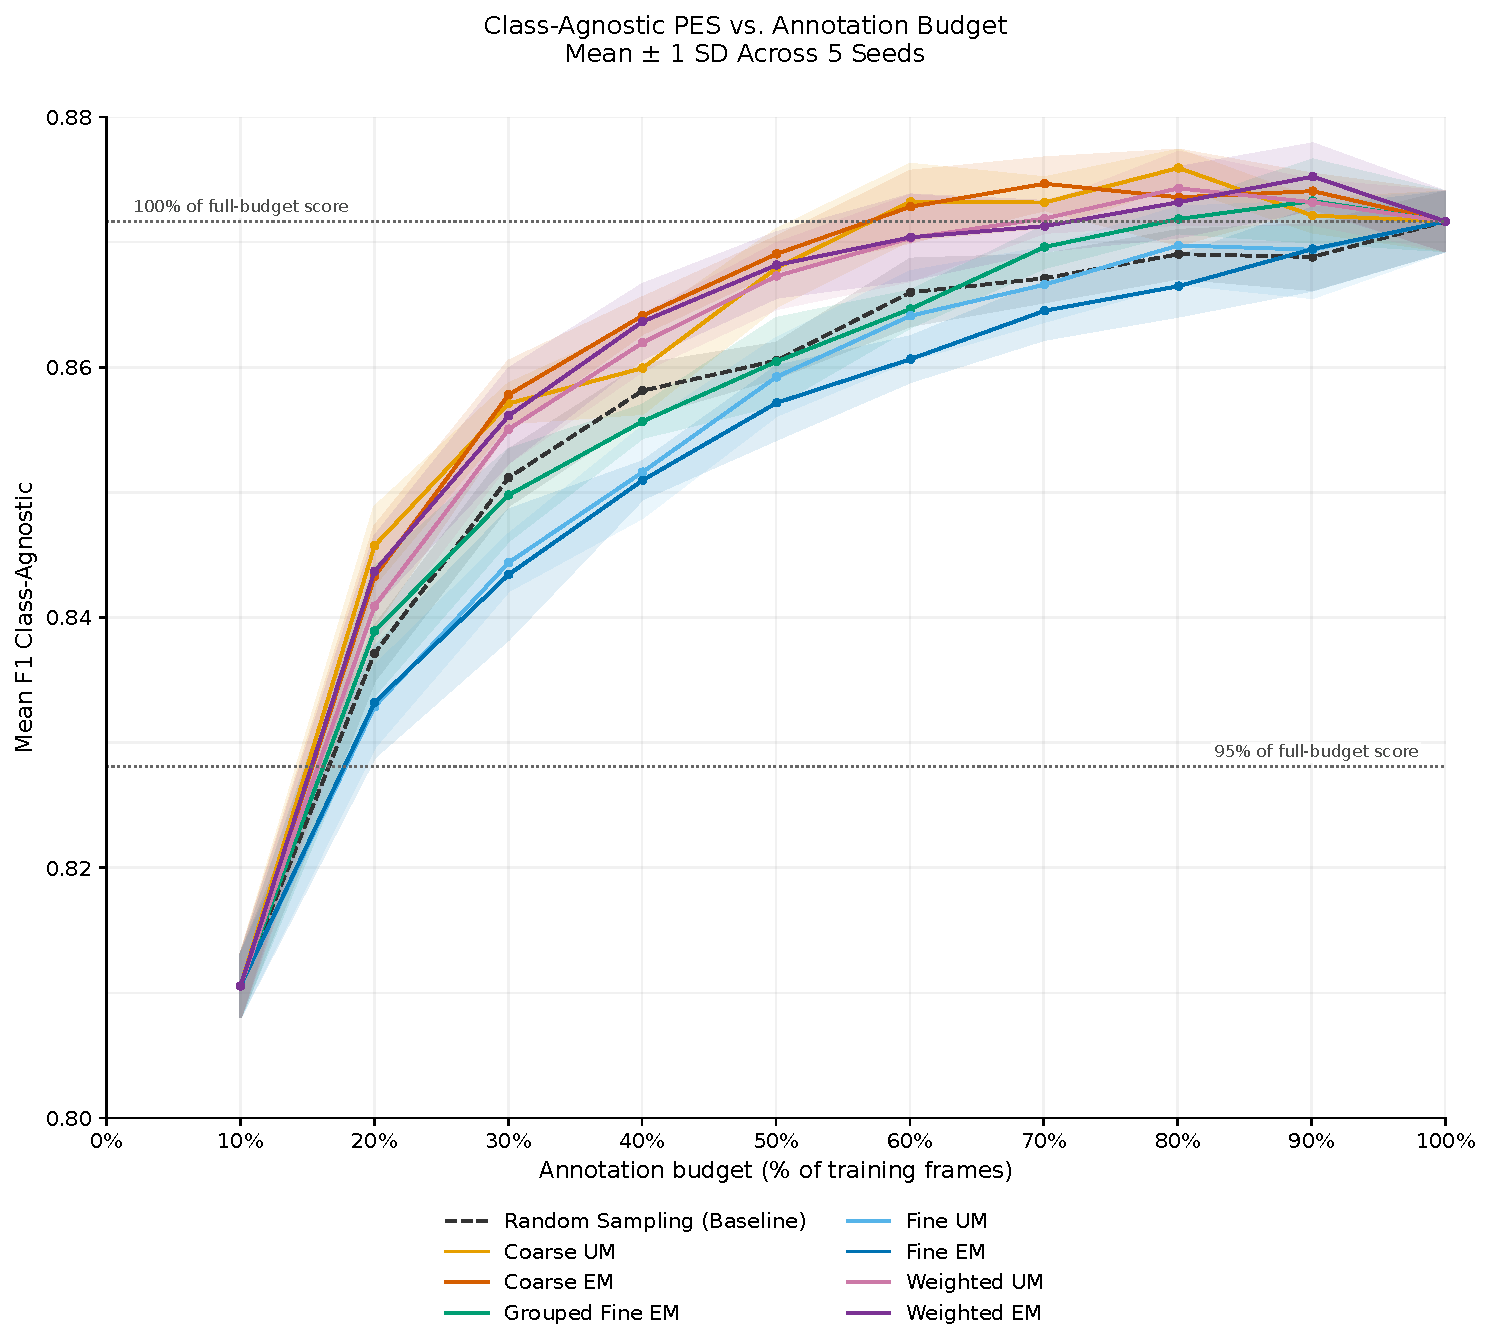
\includegraphics[width=0.85\textwidth,height=0.78\textheight,keepaspectratio]{figures/learning_curves_class_agnostic_pes.pdf}
    \caption{Class-agnostic F1 across annotation budgets. Lines show means and bands show one sample standard deviation across five seeds. Dotted lines mark fractions of the full-budget mean. Vertical axes are cropped.}
    \label{fig:Learning Curves (Mean F1 Class-Agnostic)}
\end{figure}


\begin{table}[htbp]
    \centering
    \caption{Class-agnostic AULC across query strategies. Values are mean $\pm$ sample standard deviation across five seeds, with relative changes from random sampling in parentheses. The largest mean gain is bolded.}
    \label{tab:aulc_class_agnostic}
    \small
    \begin{adjustbox}{max width=\textwidth}
        \begin{tabular}{lc}
            \toprule
            \multicolumn{2}{c}{\textbf{AULC (Class-Agnostic PES)}} \\
            \cmidrule(lr){1-2}
            \textbf{Query Strategy} & \textbf{AULC} \\
            \midrule
            R. Sampling (Baseline) & 85.77 $\pm$ 0.05 (+0.00\%) \\
            Coarse UM              & 86.29 $\pm$ 0.08 (+0.61\%) \\
            Coarse EM              & 86.34 $\pm$ 0.07 (\textbf{+0.67\%}) \\
            Fine UM                & 85.54 $\pm$ 0.07 (-0.26\%) \\
            Fine EM                & 85.41 $\pm$ 0.04 (-0.42\%) \\
            Grouped Fine EM        & 85.84 $\pm$ 0.12 (+0.08\%) \\
            Weighted UM            & 86.18 $\pm$ 0.08 (+0.48\%) \\
            Weighted EM            & 86.25 $\pm$ 0.14 (+0.57\%) \\
            \bottomrule
        \end{tabular}
    \end{adjustbox}
\end{table}

\section{Comparison Between Query Strategies}
\label{sec:Comparison Between Query Strategies}

\subsection{Event Presence and Attribute Uncertainty}
Weighted EM gives the strongest overall event-F1 results at high and medium granularity. Compared with Fine EM, it uses a soft event-probability weight over all frames instead of restricting scoring to detected events. This retains information from frames outside the detection threshold and reduces the contribution of likely background. Its advantage suggests that attribute uncertainty is more useful when combined with event presence.

Coarse strategies are also competitive despite ignoring attribute identity. Coarse UM leads event and element F1 at low granularity, and Coarse EM leads class-agnostic F1. However, their edit-score losses show that better localization is not sufficient to improve every aspect of PES.

\subsection{Grouping Attributes}
Grouped Fine EM improves on Fine EM by 1.05 and 1.07 event-F1 AULC points at high and medium granularity. Both gains occur in all five paired seeds. It also improves element F1 and class-agnostic F1, although edit-score differences are small and mixed across granularities.

The grouped score represents competition between values within each group and gives every group equal weight. This may avoid diluting uncertainty with many confidently absent attributes. The comparison supports using the label structure in acquisition, but does not isolate the effects of categorical normalization, null categories, and equal group weighting.

\subsection{UM versus EM}
There is no consistent advantage for EM. Fine UM exceeds Fine EM in all ten reported AULC comparisons. Coarse EM has small advantages at high and medium granularity for event and element F1, while Coarse UM leads at low granularity. Weighted EM improves on Weighted UM for all three event-F1 granularities, but loses edit score at high and low granularity.

UM and EM rank a single binary probability identically. Their differences here arise after averaging or weighting many predictions. Therefore, the effect of choosing entropy depends on how uncertainty is aggregated. Results also vary across datasets in \textcite{giancola_towards_2023}: EM leads the main SoccerNet-v2 comparison, while UM achieves higher AULC on the other two datasets.

\subsection{What the Strategies Acquire}
To examine possible reasons for these differences, we analyze the first four acquisition batches, which expand the initial 10\% pool to approximately 50\%. We pool the acquired clips within each seed, then average the resulting statistics across seeds. Figure~\ref{fig:Early Acquisition Composition} uses the labels of acquired clips for retrospective analysis; these labels were not used to score queries.

Coarse EM and Weighted EM acquire about 19.9 and 19.8 events per 1,000 frames, compared with 16.6 for random sampling. Fine EM acquires only 14.6. Thus, the strategies receive different numbers of labeled events at similar frame budgets. More event supervision could partly explain the gains from coarse and weighted acquisition.

The selected outcomes also differ. Winners and errors account for 20.6\% of acquired events under Coarse EM and 21.7\% under Weighted EM, compared with 27.4\% under random sampling. Less emphasis on these outcomes may contribute to weaker sequence predictions when outcome is part of the label, as in high and low granularity. This remains a hypothesis: the acquisition distributions do not directly identify which prediction errors increased.

\begin{figure}[htbp]
    \centering
    \includegraphics[width=\textwidth]{figures/early_acquisition_composition.pdf}
    \caption{Composition of the first four acquisition batches, excluding the initial pool. Bars show means and error bars show one sample standard deviation across five seeds. Dashed lines mark random sampling. Winner/error outcomes include winners, forced errors, and unforced errors.}
    \label{fig:Early Acquisition Composition}
\end{figure}
